\chapter{Revisão Bibliográfica} \label{chap:sota}


\section{Definição e caraterização do problema}\label{sec:problem}

Com a modernização constante da indústria e consequente crescente exigência
de conetividade de todo o tipo de equipamentos, é imperativa a introdução
de novas soluções tecnológicas que satisfaçam estes requisitos modernos
mas que também mantenham a compatibilidade com as exigências satisfeitas
pelos sistemas atualmente em uso.

Quando nos referimos à área da robótica, exigências temporais como o
período, a latência e a periodicidade da malha de controlo são fulcrais
para o funcionamento estável do sistema. Ora, a crescente exigência de
conetividade moderna instiga à utilização de redes de comunicação no
ambiente industrial. Quando o controlo de diversas áreas num equipamento
é feito de modo central num PLC ou micro-controlador, a sincronização de
alteração de estados de saídas é trivial, pois basta garantir que ambas
são atualizadas no mesmo ciclo de processamento. Quando se pretende
introduzir uma rede de comunicação entre o processamento central e o
controlo das saídas e/ou a aquisição das entradas, é crucial garantir
que não existem atrasos significativos na transmissão da informação
na rede e garantir a sincronização entre as atualizações das saídas
nos diversos escravos.

Nos últimos anos, várias implementações e estudos já foram realizados
com manipuladores robóticos utilizando redes de comunicação na malha de
controlo como \cite{Zhang18}, \cite{leiwang2010} ou muito recentemente
\cite{deremetz2020}. No entanto, todas elas se focam na vertente mais
industrial e técnica da solução e praticamente não existem implementações
focadas no ensino.

% económico
Um demonstrador focado no ensino deve ter caraterísticas apelativas de
modo a que a sua utilização possa ser o mais generalizada possível. O
primeiro objetivo deverá ser o desenvolvimento de um produto económico
de modo a que este possa ser adquirido em larga escala pelos
estabelecimentos de ensino. É também preciso considerar que no ambiente
de ensino, é mais provável acontecerem situações de utilização indevida
de um equipamento do que em ambiente industrial, onde geralmente apenas
pessoas qualificadas estão autorizadas a interagir com o mesmo, e portanto
uma possível avaria do produto não pode trazer prejuízos avultados à
instituição e/ou ao estudante. Naturalmente, esta redução no custo
implicará sempre uma redução na qualidade do produto final face a um
desenvolvimento de nível industrial, mas essa não é uma caraterística
fundamental de um demonstrador didático.

% implementação simples
Muitas vezes o momento em que nos é apresentada uma tecnologia desconhecida
através de um demostrador didático surgem questões acerca do demostrador
propriamente dito e não na tecnologia que ele pretende demonstrar. Assim,
para minimizar este tipo de interferência na aprendizagem existem duas
possíveis soluções: utilizar uma ideia de base que seja tão simples que
não permita qualquer tipo de dúvida ou que o público alvo tenha um
conhecimento aprofundado da ideia de base. Considerando que o público alvo
deste demostrador são estudantes de mestrado na área da robótica,
o controlo de movimento e posição de um manipulador robótico são temas
bem conhecidos.

% componentes 'off the shelf'
Complementando a caraterística económica de um demonstrador educativo,
a utilização de componentes e sub-sistemas genéricos, denominados
componentes \emph{off-the-shelf}, facilita a aquisição dos mesmos tanto
para o fabrico como para reparações. Assim, é possível que o próprio
cliente faça uma reparação do produto, sendo que a ação mais simples será
a troca do componente ou sub-sistema danificado.

% modularidade
A utilização de componentes e sub-sistemas genéricos leva-nos a um ponto
importante de demonstradores educativos: a modularidade. Um sistema
dividido em sub-sistemas mais simples que se focam numa única tarefa é um
sistema modular. Cada sub-sistema por si é simples, fácil de implementar,
interpretar e diagnosticar. A conjugação dos diferentes sub-sistemas,
encadeados e inter-ligados permite obter um sistema mais complexo com a
vantagem de que o seu desenvolvimento e eventual diagnóstico possa ser
feito por partes, o que simplifica tal processo, proporcionando também a
possibilidade de este ser paralelizado. Esta modularidade permite que,
no contexto de aprendizagem, seja mais fácil e rápido interpretar o
funcionamento de cada sub-sistema e, consequentemente, interpretar o
funcionamento geral do sistema.

% intuitivo
Por fim, a caraterística mais importante de qualquer demonstrador
educativo, e razão pela qual estes existem, é o seu caráter intuitivo.
Qualquer utilizador tem de ser capaz de, através do próprio funcionamento
do demonstrador, entender o conceito base em exposição. Em ambiente
educacional é muito importante fornecer este tipo de contacto com a
tecnologia para que os estudantes possam sedimentar os conhecimentos com
mais facilidade e de uma forma mais duradoura. % TODO arranjar citação para isto


\section{\ecat}\label{sec:ethercat}

A rede \ecat\ é uma rede de \emph{Ethernet} industrial que usa a
especificação padrão IEEE 802.3 \cite[]{ieee:IEEEStandardEthernet} para
definir o formato dos \emph{frames} e camada física a utilizar, mas
introduz uma maneira diferente de os processar.

Esta nova forma de processamento permite uma comunicação com todos os
dispositivos presentes na rede com apenas um \emph{frame}. \ecat\ utiliza
uma tipologia de comunicação \emph{Master/Slave}, tipicamente implementada
numa arquitetura de rede encadeada (\emph{daisy-chain}), mas permite várias
outras arquiteturas.
% TODO: Citar aqui algo que explicite as varias arquiteturas

\subsection{Arquiteture de rede encadeada (\emph{daisy-chain})}
\label{sec:daisychain}
Apenas o dispositivo mestre pode iniciar um \emph{frame} de comunicação
e os dispositivos escravos limitam-se a ler a parte informação contida
no \emph{frame} que lhes é endereçada. Ao mesmo tempo, cada dispositivo
escravo pode introduzir informação sua  no \emph{frame} antes de o enviar
para o dispositivo seguinte.

\subsection{sincronização de relógios}
% TODO

\subsection{Conclusão}
Estas caraterísticas permitem que o dispositivo mestre seja implementado
em qualquer tipo de dispositivo que contenha uma porta de comunicação 
\emph{Ethernet}. Os dispositivos escravo utilizam um \emph{EtherCAT Slave
Controller} (ESC) que processa os \emph{frames} fazendo com que a velocidade
e tempos de resposta da rede sejam previsíveis e independentes dos 
dispositivos escravo que existam na rede. Assim, é possível a utilização
de dispositivos escravo implementados em arquiteturas de computação
diferentes dentro da mesma rede \ecat.


\section{Soluções propostas} \label{sec:solution}

Para atingir os objetivos propostos por esta dissertação, foram propostas 
duas possíveis soluções. Ambas são apresentadas de seguida sendo que
maior ênfase será dada na última, pois é a proposta que se mostra mais
adequada ao estudo em questão.

Ambas as soluções têm por base o controlo de movimento através da velocidade
e/ou posição de um sistema robótico de múltiplos eixos. Fazendo uso de
uma arquitetura de controlo distribuída interligada por uma rede \ecat\
em tipologia encadeada (secção \ref{sec:daisychain}). Esta arquitetura
será constituída por um dispositivo mestre implementado num micro-computador
\raspi\, programado através das linguagens descritas no padrão
IEC 61161-3. Os dispositivos escravo, que farão a interface com os atuadores,
sensores e interface de comando, serão implementados através de placas
\arduino\ agrupado com o adaptador \emph{EasyCAT} da \cite{ABT:EasyCAT}.
Um esquema da arquitetura pretendida é mostrado na figura
\ref{fig:network-architecture}.

\begin{figure}
 \centering
 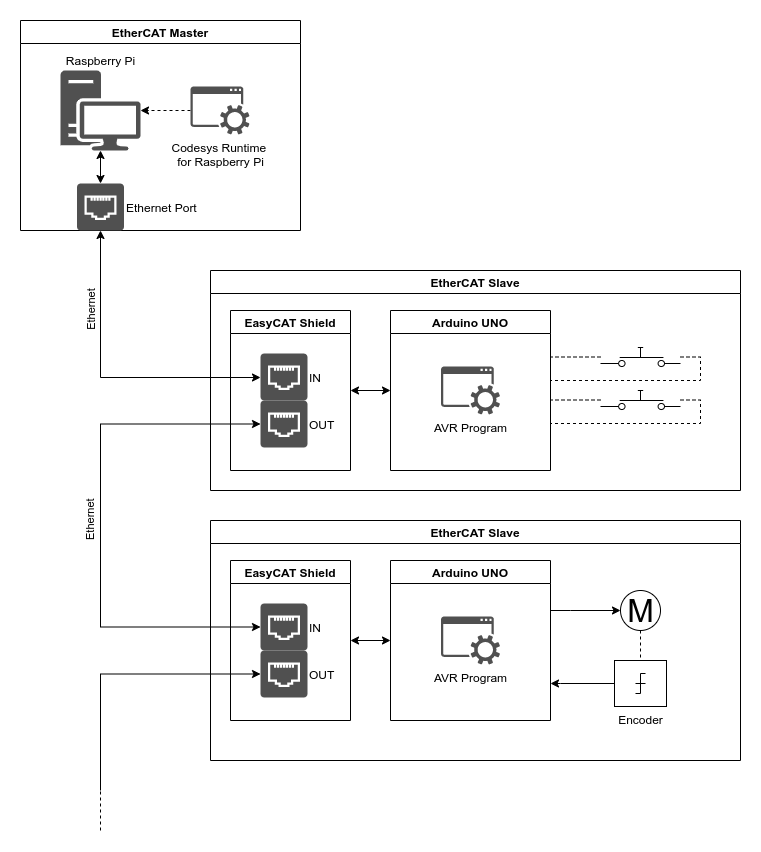
\includegraphics[width=\linewidth]{network-diagram_transparent.png}
 \caption{Arquitetura da rede \ecat\ pretendida}
 \label{fig:network-architecture}
\end{figure}



\subsection{Controlo de discos perfurados}\label{sec:discs_project}

%\subsubsection{O conceito}
A primeira solução idealizada no contexto desta dissertação baseia-se num
sistema de controlo e sincronização de discos rotativos independentes.
Estes são perfurados na extremidade de maneira a que possam ser momentaneamente atravessados por um feixe de laser. Este último será fixo numa das extremidades
do demonstrador com orientação que permita atravessar todos os discos presentes
no sistema, ficando visível na extremidade oposta do demonstrador. Assim,
com estes discos acoplados a motores DC com codificadores de posição (\emph{encoder}),
controlados de forma independente por placas \arduino\ a funcionar em modo
de \ecat\ \emph{slave}, é possível criar diferentes cenários de controlo
cujo objetivo seja periodicamente alinhar as furações dos discos com o
feixe laser, permitindo que este seja viaje até à extremidade oposta.

Para complementar este conceito, será necessário permitir que o estado
do ponteiro laser (ligado ou desligado) seja controlado pelo sistema,
criando uma camada adicional de complexidade que ajuda a entender a
importância da sincronização de relógios nas redes de comunicação de
tempo real. Desta forma é possível ativar o ponteiro laser apenas quando
o sistema  determinar que os discos estão na orientação correta, fazendo
com seja mais percetível a importância da sincronização de relógios para
que seja possível uma atualização síncrona do estado das saídas.

%\subsubsection{Flexibilidade}
Idealmente esta soluçao deverá permitir efetuar o mesmo controlo mas não
usando as capacidades da rede \ecat\ e usando apenas comunicação
\emph{Ethernet} simples, o que permitirá efetuar uma comparação efetiva
destes protocolos e demonstrar que em ambientes de rede de comunicação
tradicionais não existem considerações de tempo real nem de sincronização.
Esta funcionalidade implicará verificar se os adaptadores \emph{EasyCAT}
permitem comunicação \emph{Ethernet} simples ou até de outros protocolos
de \emph{Ethernet} industrial (p.ex. \emph{Modbus TCP}), mas até ao momento
ainda não o foi possível determinar.

%\subsubsection{Conclusão}
Desta forma evidenciam-se as capacidades da rede \ecat\ no que diz
respeito à resposta temporal, sincronização de relógios e capacidade de
transferência de dados num sistema cujo conceito é acessível a qualquer
estudante de engenharia eletrotécnica.


\subsection{Seguimento de um traçado com um braço robótico}\label{sec:robotic_arm}

% \subsubsection{O conceito}
A segunda proposta de solução para a dissertação em estudo trata-se do
controlo de um manipulador robótico do tipo 'braço' através da mesma
arquitetura de comunicação e de controlo descrita em \ref{sec:solution} e
\ref{sec:discs_project}. O objetivo deste braço robótico será fazer o
seguimento de um caminho, do estilo labirinto, com a sua ferramenta.
Esta poderá ser, por exemplo, um apontador laser (derivado do conceito
descrito em \ref{sec:discs_project}) ou, no caso de verificar viável, uma
massa de esparguete.

A utilização de um objeto tridimensional como ferramenta torna a ação de
percorrer um trajeto mais interessante e relevante para o objetivo.
Quando se considera a utilização de um apontador laser, este só tem
representação num plano bidimensional e portanto pode ser usada uma folha
de papel como suporte para o trajeto. Considerando a utilização de um
objeto tridimensional como ferramenta, como é o caso da massa de
esparguete, torna-se necessária a utilizaçao de um suporte tridimensional
com canais para definir o trajeto. No âmbito deste projeto, um suporte
em material como plástico PLA ou MDF é suficiente para atingir os objetivos
propostos.

% Esta última pode deixar alguma confusão no leitor mas
% é preciso pensar um pouco 'fora da caixa': se o caminho a ser percorrido
% for definido por canais abertos num suporte tridimensional, é possível 
% utilizar um objeto bidimensional para o percorrer.

% \subsubsection{Conclusão}

